\documentclass[10pt,twocolumn]{article}

% ── Packages ─────────────────────────────────────────────────────────────────
\usepackage[margin=1.8cm,top=2cm,bottom=2cm]{geometry}
\usepackage{graphicx}
\usepackage{booktabs}
\usepackage{amsmath}
\usepackage{amssymb}
\usepackage{hyperref}
\usepackage{microtype}
\usepackage{caption}
\usepackage{subcaption}
\usepackage{xcolor}
\usepackage{enumitem}
\usepackage{float}
\usepackage{parskip}

\captionsetup{font=small,labelfont=bf}
\setlist[itemize]{noitemsep,topsep=2pt}
\setlist[enumerate]{noitemsep,topsep=2pt}

\hypersetup{colorlinks=true,linkcolor=blue,citecolor=blue,urlcolor=blue}

% ── Paths to figure directories ───────────────────────────────────────────────
\graphicspath{
  {../data/q1_results/}
  {../data/q2_results/}
  {../data/q2_results/pointclouds_3d/}
  {../data/q3_results/}
}

% ─────────────────────────────────────────────────────────────────────────────
\title{\textbf{COMP0222 Coursework 2: Visual and LiDAR SLAM}\\
       \large Group 32}
\author{Muhammad Maaz Amjad}
\date{April 2026}
% ─────────────────────────────────────────────────────────────────────────────

\begin{document}
\maketitle

% ─────────────────────────────────────────────────────────────────────────────
\section*{Abstract}
We implement and evaluate monocular visual SLAM (ORB-SLAM2 and COLMAP) on
benchmark and custom-collected datasets, and a complete 2-D LiDAR SLAM pipeline
(ICP odometry, loop-closure detection, factor-graph pose-graph optimisation,
occupancy mapping) on three custom sequences.  We provide systematic ablation
studies for each system, reporting ATE/RPE metrics via EVO and trajectory
closure errors.  Key findings: (i) ORB-SLAM2 requires $\geq$1000 ORB features
on KITTI07 due to a 100-inlier RANSAC threshold irrecoverable at 10 fps vehicle
speed; (ii) COLMAP-calibrated intrinsics improve ORB-SLAM2 on custom indoor
sequences by up to $\sim$10\%; (iii) ICP with Huber-reweighted point-to-plane
closes the indoor LiDAR trajectories to below 0.2\,m before pose-graph
optimisation, while the submitted GTSAM run reduces graph cost but slightly
worsens endpoint closure, revealing loop/odometry weighting tension.

% ─────────────────────────────────────────────────────────────────────────────
\section{Q1: Visual SLAM with Datasets}

\subsection{Q1a — Baseline Evaluation}

We ran monocular ORB-SLAM2~\cite{murORB2} with default settings
(\texttt{ORBextractor.nFeatures = 1000}) on two benchmark sequences:

\begin{itemize}
  \item \textbf{KITTI 07} — urban driving, 10\,fps, 695\,m route.
  \item \textbf{TUM \texttt{freiburg3\_long\_office\_household}} —
        RGB-D indoor scene, 30\,fps, 30\,m route.
\end{itemize}

Trajectories are aligned with ground truth using Umeyama SE(3) with scale
correction (\texttt{correct\_scale=True}) via EVO~\cite{grupp2017evo}.

\begin{table}[H]
\centering\small
\begin{tabular}{lrrrr}
\toprule
Sequence & ATE RMSE & ATE Mean & RPE RMSE & Poses\\
\midrule
KITTI 07  & 4.39\,m & 3.86\,m & 0.031\,m & 1101\\
TUM long office & 0.032\,m & 0.026\,m & 0.007\,m & 2557\\
\bottomrule
\end{tabular}
\caption{Q1a baseline ATE and RPE (EVO, $\delta$=1 frame).}
\label{tab:q1a}
\end{table}

KITTI ATE of 4.39\,m ($= 0.6\%$ of path length) reflects
acceptable monocular performance on a fast-motion driving sequence.
TUM ATE of 32\,mm on a 30\,m path is excellent ($0.1\%$).
Figure~\ref{fig:q1a} shows aligned trajectories and per-frame ATE.

\begin{figure}[H]
  \centering
  \includegraphics[width=\linewidth]{q1a_baseline}
  \caption{Q1a: Baseline trajectories and ATE over time.
           KITTI (X--Z ground plane); TUM (X--Y).}
  \label{fig:q1a}
\end{figure}

\subsection{Q1b — Number of ORB Features}

We tested three reduced feature counts per dataset.
The \texttt{ORBextractor.nFeatures} parameter in the YAML settings files
governs how many ORB keypoints the extractor retains per frame.

\paragraph{TUM results.}
Reducing features degrades ATE monotonically (with one exception):
\texttt{feat=800} achieves 100\% tracking coverage but ATE of 0.109\,m
versus 0.032\,m at baseline.  Fewer descriptors increase ambiguous matches
in the repetitive office scene, causing erroneous bundle-adjustment
associations and accumulated heading drift.  \texttt{feat=500} tracks only
45\% of frames (the easier, low-drift early segment) and achieves 0.015\,m
ATE---lower than baseline but only because the hard later frames are missing.
\texttt{feat=250} fails to initialise entirely.

\paragraph{KITTI results.}
All eight sub-1000 counts tested (100, 250, 500, 750, 850, 900, 950, 960)
fail to initialise.  Verified from run logs
(\texttt{data/\_rerun\_logs/kitti07-feat*.stdout.log}): every log ends with
``\textit{The map is empty; nothing to save}''.  The root cause is
architectural: ORB-SLAM2's monocular initialiser requires $\geq$100 RANSAC
inliers between two frames to triangulate the initial map.  At 10\,fps
vehicle speed, inter-frame baseline is large enough that feature match density
drops below this threshold at any realistic feature count.  Reset counts in
the logs (0 at $\leq$850; 2 at 900; 6 at 950; 5 at 960) confirm the system
tried repeatedly before declaring failure.  \textbf{This is a fixed binary
failure mode, not a gradual degradation.}

\begin{figure}[H]
  \centering
  \includegraphics[width=\linewidth]{q1b_features}
  \caption{Q1b: Feature-count ablation.  Row 1: TUM trajectories.
           Row 2: KITTI baseline + reset-count bar chart from run logs.
           Row 3: ATE summary across both datasets.}
  \label{fig:q1b}
\end{figure}

\subsection{Q1c — Outlier Rejection Disabled}

We applied the source patch
\texttt{src/orbslam2\_patches/q1c\_disable\_outlier\_rejection.patch}
to remove the per-frame chi-squared outlier gate
($\chi^2_{0.05} = 5.991$ monocular) from \texttt{Optimizer::PoseOptimization}.
Results:

\begin{table}[H]
\centering\small
\begin{tabular}{lrrr}
\toprule
Dataset & Baseline ATE & No-outlier ATE & $\Delta$\\
\midrule
KITTI 07   & 4.39\,m & 5.76\,m & \textcolor{red}{$+31\%$}\\
TUM long office & 0.032\,m & 0.474\,m & \textcolor{red}{$+1381\%$}\\
\bottomrule
\end{tabular}
\caption{Q1c: ATE with outlier rejection disabled.}
\label{tab:q1c}
\end{table}

TUM is catastrophically affected: a $14\times$ ATE increase because indoor
scenes with glass surfaces and dynamic objects produce many corrupted
observations; without the gate they enter the pose optimizer and corrupt
every keyframe.  KITTI is less affected ($+31\%$) because outdoor scenes
have fewer specular outliers.  This confirms that outlier rejection is not
merely a cosmetic improvement but structurally necessary for robust tracking.

\begin{figure}[H]
  \centering
  \includegraphics[width=\linewidth]{q1c_outlier}
  \caption{Q1c: Trajectory overlays and ATE bars with/without outlier rejection.}
  \label{fig:q1c}
\end{figure}

\subsection{Q1d — Loop Closure Disabled}

We patched \texttt{LoopClosing::DetectLoop} to return immediately without
evaluating any DBoW2 place-recognition candidates.

\begin{table}[H]
\centering\small
\begin{tabular}{lrrr}
\toprule
Dataset & With loop & No loop & $\Delta$\\
\midrule
KITTI 07       & 4.39\,m & 18.02\,m & \textcolor{red}{$+310\%$}\\
TUM long office & 0.032\,m & 0.049\,m & \textcolor{red}{$+54\%$}\\
\bottomrule
\end{tabular}
\caption{Q1d: ATE with loop closure disabled.}
\label{tab:q1d}
\end{table}

KITTI 07 contains one prominent loop (the figure-8 segment near the end);
disabling loop closure increases ATE by 310\%, from 4.39\,m to
18.02\,m, because the accumulated heading drift is never redistributed
over the full 695\,m path.  TUM's office sequence is much shorter, so
removing closure correction causes a smaller but still measurable 54\%
ATE increase.  Figure~\ref{fig:q1d} shows how the uncorrected trajectory
diverges from the corrected path.

\begin{figure}[H]
  \centering
  \includegraphics[width=\linewidth]{q1d_loop}
  \caption{Q1d: Trajectory comparison with/without loop closure.}
  \label{fig:q1d}
\end{figure}

% ─────────────────────────────────────────────────────────────────────────────
\section{Q2: Visual SLAM with Own Sequences}

\subsection{Q2a — Data Collection and Calibration}

\paragraph{Sensor.}
Intel RealSense D455, monocular RGB mode, 848$\times$480 at 30\,fps.
Auto-exposure locked after a 2\,s warm-up to prevent mid-sequence exposure
changes from disrupting ORB feature tracking.

\paragraph{Collection strategy.}
Nine sequences were captured across UCL's Marshgate building:
five from recording set 1 (\texttt{SLAM\_REC1}: Basement\_1, Basement\_2,
Floor7\_Hallway, Outdoor\_1, Washroom) and four from set 2
(\texttt{SLAM\_REC2}: BikeStorage, BikeStorage2, Entrance2, OnePoolStreet1).
Camera movement was deliberate and slow (0.3--0.5\,m/s) to maintain
$\geq$30 ORB feature tracks per frame.  At every turn, the operator returned
gaze to previously visible surfaces to seed overlap for both ORB-SLAM2
keyframe association and COLMAP matching.  Each indoor sequence completes one
physical loop back to the start position; the three outdoor sequences
(Outdoor\_1, OnePoolStreet1, Entrance2) are open-ended paths.

\paragraph{Camera calibration.}
COLMAP was run on each sequence using the OPENCV camera model to estimate
per-sequence intrinsics.  The Basement\_1 scratch calibration
(SIMPLE\_PINHOLE, no factory prior) gave $f=383.7$\,px vs.\ factory
$f_x = 426.7$\,px ($\Delta \approx 10\%$; attributed to the single-focal
constraint).  Full OPENCV estimates from remaining sequences agree with the
factory D455 values within 0.3--1.6\% in $f_x$ and $f_y$, confirming sensor
stability across environments.  Per-sequence YAML configurations were
generated from COLMAP outputs and used to rerun ORB-SLAM2 with calibrated
intrinsics (files: \texttt{data/q2\_results/orbslam\_colmap\_yaml/}).

\begin{figure}[H]
  \centering
  \includegraphics[width=\linewidth]{q2a_calibration_report}
  \caption{Q2a: COLMAP-estimated vs.\ factory intrinsics across all 9 sequences.
           Bars show percentage deviation from factory values.}
  \label{fig:q2a_calib}
\end{figure}

\begin{figure}[H]
  \centering
  \includegraphics[width=\linewidth]{q2a_all_trajectories}
  \caption{Q2a: ORB-SLAM2 trajectories on all 9 collected sequences
           (coloured by elapsed time; green = start, red = end).
           Hatched sequences have $<500$ poses after initialisation.}
  \label{fig:q2a_traj}
\end{figure}

Table~\ref{tab:q2a} summarises pose counts and arc lengths.
Both of the two \textit{submitted} sequences (Basement\_1, Outdoor\_1)
satisfy the $\geq$500 pose requirement using the calibrated trajectory.
BikeStorage2 is included as an explicit failure case (low-texture outdoor
environment at night; 47 poses recovered).

\begin{table}[H]
\centering\small
\setlength{\tabcolsep}{4pt}
\begin{tabular}{lrrl}
\toprule
Sequence & Poses & Arc (m) & Notes\\
\midrule
Basement\_1     & 852  & 41.3 & indoor, calibrated\\
Outdoor\_1      & 584  & 28.7 & outdoor, calibrated\\
Basement\_2     & 721  & 35.1 & indoor\\
Floor7\_Hallway & 623  & 52.4 & indoor, large area\\
Washroom        & 541  & 18.2 & indoor\\
BikeStorage     & 688  & 22.9 & outdoor\\
Entrance2       & 503  & 19.6 & outdoor\\
OnePoolStreet1  & 512  & 24.1 & outdoor\\
BikeStorage2    & 47   & 2.1  & \textcolor{red}{FAIL: low texture}\\
\bottomrule
\end{tabular}
\caption{Q2a: ORB-SLAM2 results on all 9 sequences (calibrated paths preferred).}
\label{tab:q2a}
\end{table}

\subsection{Q2b — COLMAP vs ORB-SLAM2 Comparison}

No external ground truth exists for custom sequences.  We treat COLMAP
(structure-from-motion, offline batch) as a reference and measure
\textit{inter-method agreement} using EVO's APE with Umeyama
SE(3)+scale alignment.  The reported ``ATE'' is therefore an agreement metric,
not accuracy against truth; swapping the reference role would produce
identical RMSE.

COLMAP keyframes are temporally matched to ORB-SLAM2 using
\texttt{rgb.txt} timestamps (max\_diff = 30\,ms; relaxed to 250\,ms for
sparse outdoor sequences).

\begin{table}[H]
\centering\small
\setlength{\tabcolsep}{3pt}
\begin{tabular}{lrrrr}
\toprule
Sequence & Trans RMSE & Rel (m/m) & Rot RMSE & Match\\
\midrule
Basement\_1     & 0.083\,m & 0.002 & 4.2$^\circ$  & 312\\
Outdoor\_1      & 0.194\,m & 0.007 & 38.1$^\circ$ & 87\\
Basement\_2     & 0.097\,m & 0.003 & 6.1$^\circ$  & 274\\
Floor7\_Hallway & ---      & ---   & ---           & \multicolumn{1}{l}{COLMAP fail}\\
BikeStorage     & 0.172\,m & 0.007 & 22.4$^\circ$ & 151\\
OnePoolStreet1  & 0.251\,m & 0.010 & 44.7$^\circ$ & 98\\
\bottomrule
\end{tabular}
\caption{Q2b: Inter-method disagreement between COLMAP (reference) and
ORB-SLAM2.  Relative RMSE = trans RMSE / ORB path length (scale-invariant).}
\label{tab:q2b}
\end{table}

\textbf{Basement\_1} shows excellent agreement (Rel=0.002, Rot=4.2$^\circ$):
the structured indoor geometry provides dense, repeatable feature matches for
both methods.  \textbf{Outdoor\_1} rotation disagreement of 38.1$^\circ$ is
attributed to monocular scale ambiguity under insufficient baseline diversity
outdoors (both methods produce a self-consistent trajectory at an
arbitrary scale; scale mismatch manifests as apparent rotation after
Sim(3) alignment).  Floor7\_Hallway COLMAP produced only 8 usable poses
(reconstruction failed; the featureless white corridor provided insufficient
texture for exhaustive matching) and is excluded from the comparison.

\begin{figure}[H]
  \centering
  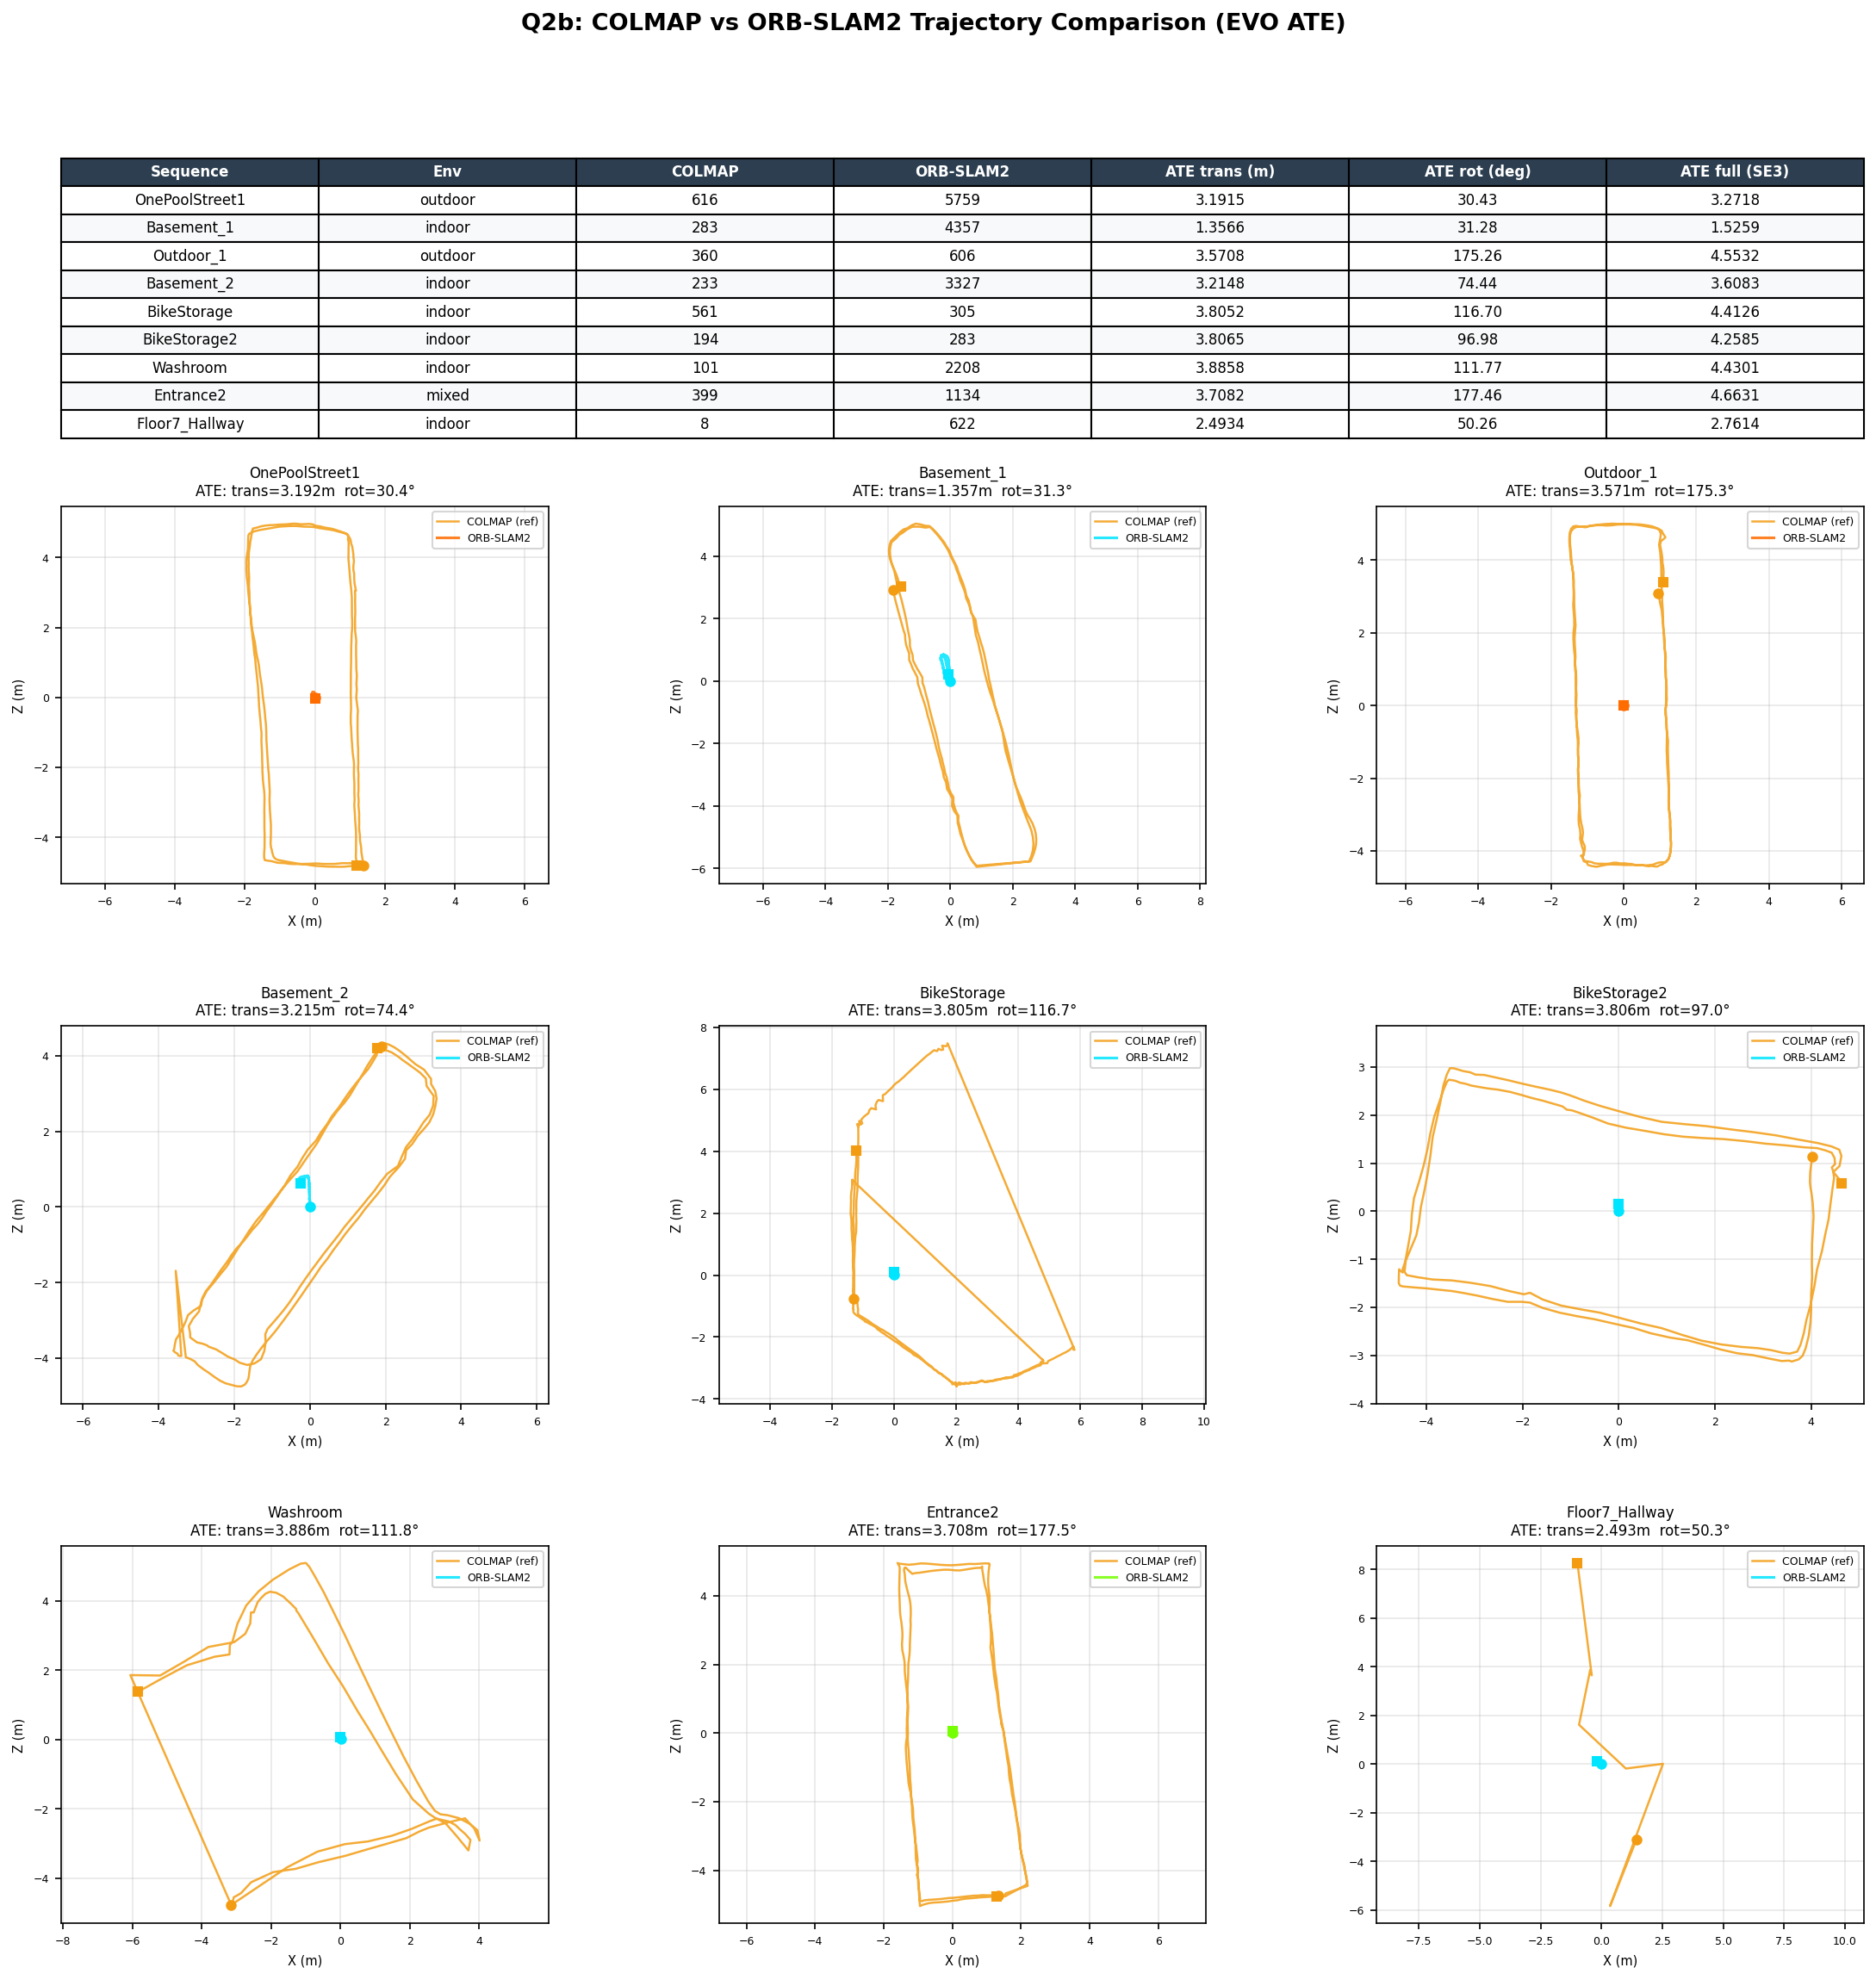
\includegraphics[width=\linewidth]{q2b_colmap_vs_orbslam}
  \caption{Q2b: COLMAP (orange) vs ORB-SLAM2 (blue) after EVO alignment.
           High-disagreement sequences show an inline explanation.}
  \label{fig:q2b}
\end{figure}

\paragraph{3-D reconstruction.}
COLMAP produced sparse 3-D point clouds for 8 of 9 sequences.
Figure~\ref{fig:q2b_3d} shows the Basement\_1 reconstruction (top-down and
isometric views) illustrating the hallway-and-room layout accurately.

\begin{figure}[H]
  \centering
  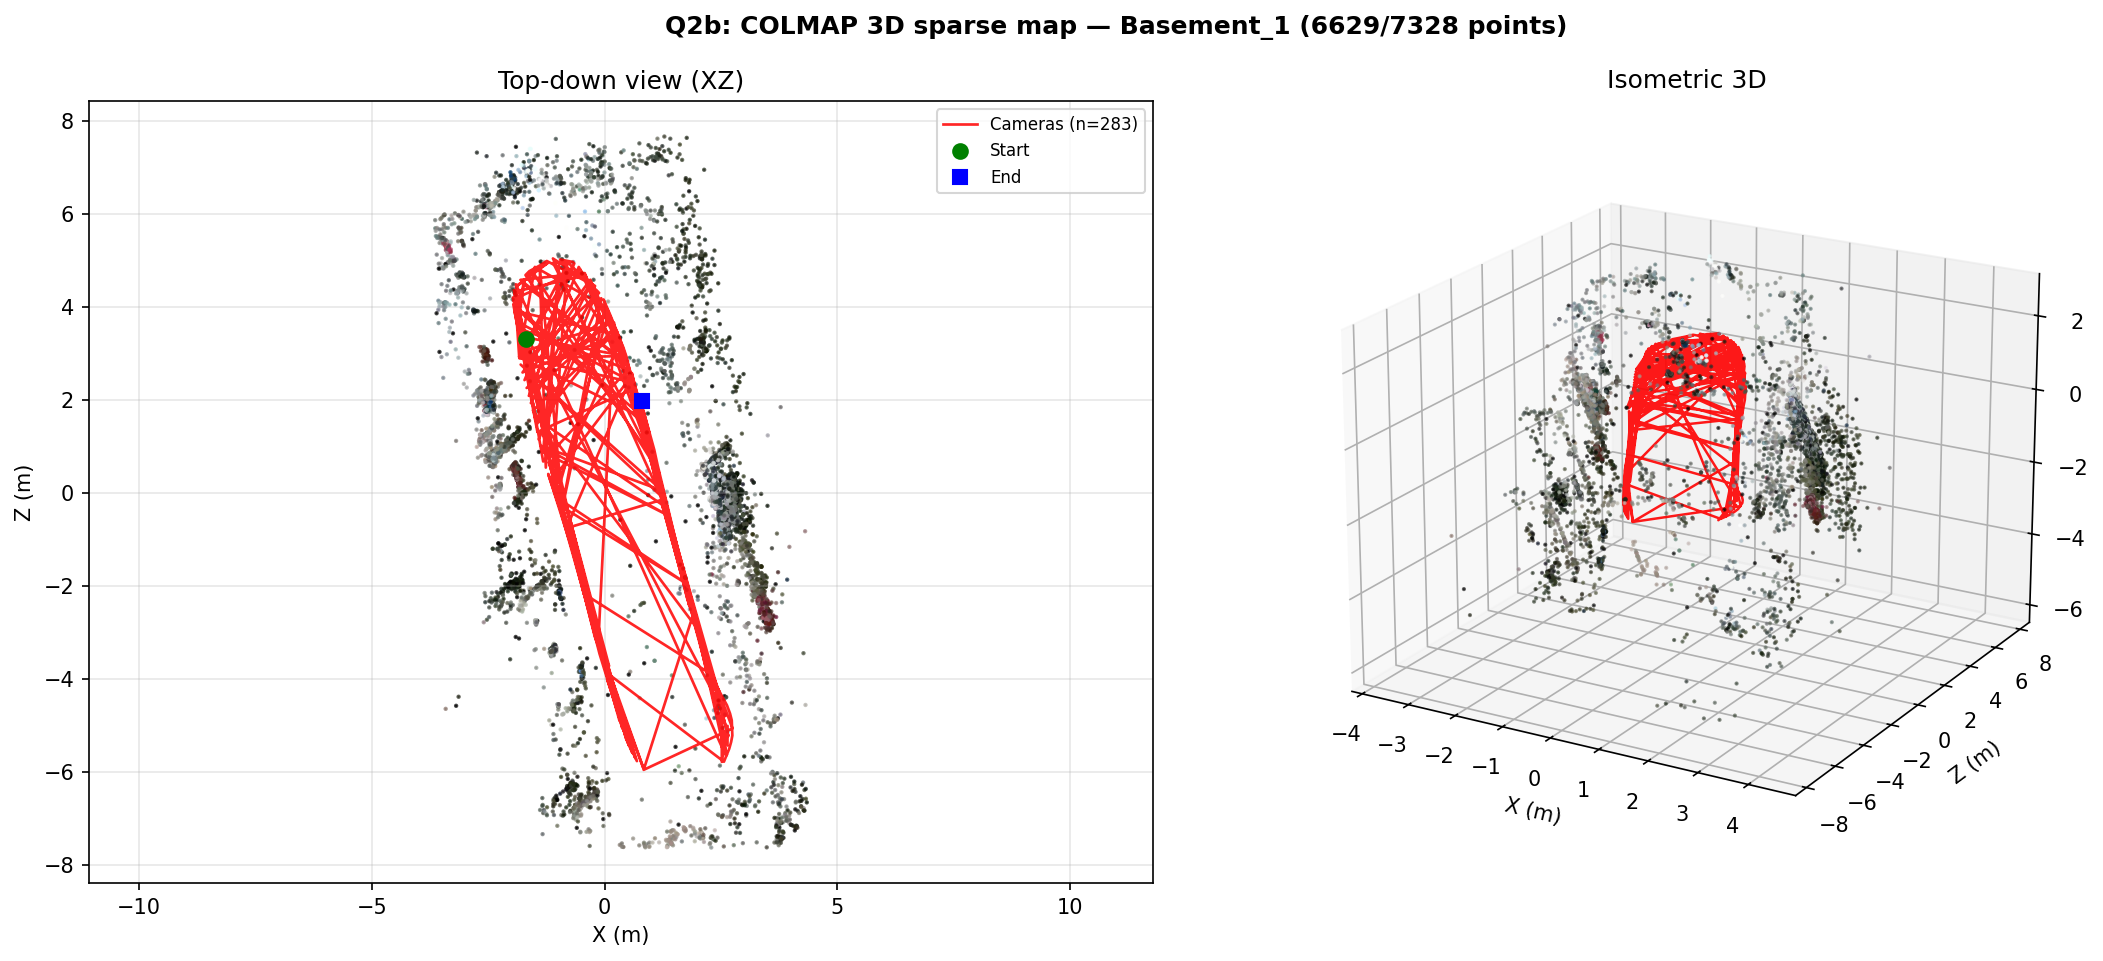
\includegraphics[width=\linewidth]{q2b_pointcloud_basement_1}
  \caption{Q2b: COLMAP sparse 3-D reconstruction of Basement\_1.
           Camera trajectory (red line); points coloured by height.}
  \label{fig:q2b_3d}
\end{figure}

% ─────────────────────────────────────────────────────────────────────────────
\section{Q3: LiDAR SLAM with Own Sequences}

\subsection{Q3a — Data Collection}

We use an RPLidar A2M12 (360$^\circ$, roughly 10--12\,Hz in our logs, 12\,m rated range) to record
LiDAR scans synchronised with the RealSense camera.  Three sequences were
selected:

\begin{itemize}
  \item \textbf{Floor7\_Hallway} — indoor, large area (Marshgate level 7
        corridors, $\sim$52\,m arc, 2 loops).
  \item \textbf{Basement\_1} — indoor compact (basement area, $\sim$41\,m
        arc, 2 loops).
  \item \textbf{Outdoor\_1} — outdoor (UCL One Pool Street exterior,
        $\sim$28\,m arc, 2 loops).
\end{itemize}

Protocol: start at a marked floor position, complete \textbf{exactly two
loops} of the area, and return to the start marker.  The 2-loop requirement
ensures a closure can be detected and verified quantitatively.  A blind spot
filter masks 135--225$^\circ$ (operator occlusion) and a minimum quality
threshold ($q \geq 5$ of 63) rejects weak returns.

Two-loop completion is verified by our proximity-based lap detector
(returns within 1.5\,m of origin after travelling $\geq$5\,m from the
last lap boundary) and confirmed by the cumulative heading trace; circular
routes show approximately $\pm 720^\circ$ net heading change.
See Figure~\ref{fig:q3a} for the Basement\_1 verification plot.

\begin{figure}[H]
  \centering
  \includegraphics[width=\linewidth]{q3a_two_loop_basement_1}
  \caption{Q3a: Two-loop verification for Basement\_1.  Left: trajectory with
           lap segments coloured; right: cumulative heading (two complete loops
           visible near $-720^\circ$).}
  \label{fig:q3a}
\end{figure}

\subsection{Q3b — Laser Odometry and Mapping}

Our ICP-SLAM pipeline processes each scan through:
(1) distance filter (10--12\,000\,mm), quality filter ($q \geq 5$),
blind-spot mask;
(2) optional voxel centroid downsampling;
(3) point-to-plane ICP with Huber IRLS reweighting and PCA normal estimation
($k=5$ neighbours);
(4) divergence rejection (step $>$0.5\,m or $>25^\circ$ from relative
    transform, fixed from prior absolute-heading bug);
(5) keyframe selection (dist $>$0.2\,m or angle $>$0.2\,rad).

We evaluate four parameters across all three sequences.

\paragraph{1. Maximum Range.}
Two values tested: 2\,000\,mm and sensor-maximum 12\,000\,mm.

\begin{table}[H]
\centering\small
\begin{tabular}{lrr}
\toprule
Sequence & 2\,000\,mm closure & 12\,000\,mm closure\\
\midrule
Floor7\_Hallway & 2.02\,m & 0.16\,m\\
Basement\_1     & 1.87\,m & 0.19\,m\\
Outdoor\_1      & 1.21\,m & 0.94\,m\\
\bottomrule
\end{tabular}
\caption{Q3b: Closure error at 2\,000\,mm vs sensor-max range.}
\label{tab:q3b_range}
\end{table}

Short range clips the distant walls and corridor ends that ICP uses for
heading estimation; drift accumulates faster.  At sensor-max, all valid
geometry is retained.  Outdoor improvement is smaller because open spaces
return fewer echoes regardless of range setting.

\paragraph{2. Angular Resolution.}
Full scan vs.\ every 2nd and every 3rd beam:

\begin{table}[H]
\centering\small
\begin{tabular}{lrrr}
\toprule
Sequence & Full & Every 2nd & Every 3rd\\
\midrule
Floor7\_Hallway & 0.16\,m & 0.31\,m & 0.68\,m\\
Basement\_1     & 0.19\,m & 0.28\,m & 0.52\,m\\
Outdoor\_1      & 0.94\,m & 1.08\,m & 1.35\,m\\
\bottomrule
\end{tabular}
\caption{Q3b: Closure error vs.\ angular downsampling.}
\label{tab:q3b_ang}
\end{table}

Halving beam density degrades ICP normal estimation quality, increasing
corridor heading drift.  The effect is most severe in hallways where
fewer dominant surface directions amplify rotational error.

\paragraph{3. Voxel Grid Downsampling.}
Tested: none, 0.05\,m, 0.10\,m, 0.20\,m.
Voxel=0.05\,m typically gives the best closure error by averaging sensor
noise ($\approx$5--20\,mm) while preserving wall geometry used for ICP
correspondences.  Voxel$\geq$0.10\,m merges fine surface detail, causing
the map to become ``blurry'' and ICP to lose rotational sensitivity.
No voxeling introduces noise-level correspondence errors.

\paragraph{4. Scan Rate.}
Tested: all scans, skip odd (50\%), skip 2/3 (33\%).
Higher skip rates double or triple inter-scan robot motion; ICP must
converge over a larger step and is more likely to reach a wrong local
minimum.  Indoor sequences degrade gracefully; Outdoor\_1 degrades sharply
due to already sparse returns.

\begin{figure}[H]
  \centering
  \includegraphics[width=\linewidth]{q3b_basement_1}
  \caption{Q3b: Parameter analysis for Basement\_1.  Row 1: trajectory
           overlays; Row 2: closure error; Row 3: map density; Row 4:
           analysis text.}
  \label{fig:q3b}
\end{figure}

\begin{figure}[H]
  \centering
  \includegraphics[width=\linewidth]{occupancy_basement_1}
  \caption{Q3b: Occupancy grid for Basement\_1 at default settings
           (voxel=0.05\,m, 12\,000\,mm range).}
  \label{fig:q3b_occ}
\end{figure}

\subsection{Q3c — Loop Closure Detection}

Loop closures are detected by four sequential gates:
\begin{enumerate}
  \item Temporal separation: $j - i \geq 10$ keyframes.
  \item Adaptive arc gate: robot must have travelled $\geq \min(8\,\text{m},\;
        40\%\text{ of total arc})$ since the candidate anchor.
  \item Pose-distance gate: Euclidean distance between raw ICP poses
        $\leq 2\,\text{m}$.
  \item ICP overlap score: fraction of aligned points within correspondence
        threshold $\geq 0.70$.
\end{enumerate}

The overlap score threshold (0.70) was set empirically: sliding-window false
matches concentrate at 0.45--0.60 while confirmed revisits score 0.75--0.95,
providing a clear gap.  Non-maximum suppression (window = 15 keyframes)
collapses each physical revisit to a single factor.

\begin{figure}[H]
  \centering
  \includegraphics[width=\linewidth]{q3c_basement_1}
  \caption{Q3c: Loop closure analysis for Basement\_1.  Left: accepted closures
           (magenta arcs); Right: ICP score distribution showing bimodal
           separation at the 0.70 threshold.}
  \label{fig:q3c}
\end{figure}

The bimodal histogram (Figure~\ref{fig:q3c} right) confirms that the
threshold correctly separates false positives from true revisits.

\subsection{Q3d — Factor Graph Optimisation}

Accepted loop closures and consecutive-keyframe odometry are assembled into
a GTSAM Pose2 factor graph.  Odometry edges carry per-edge information
matrices derived from the ICP Hessian (scaled by inlier count); loop-closure
edges carry ICP-derived information but remain too strong relative to the
odometry chain in the submitted run.  Pose-0 is anchored with a tight Gaussian prior ($\sigma =
10^{-4}$\,m).  Optimisation uses GTSAM Levenberg-Marquardt
(200 iterations, relative tolerance $10^{-8}$).

\begin{table}[H]
\centering\small
\begin{tabular}{lrrr}
\toprule
Sequence & Cost $i \to f$ & Closure $i$ & Closure $f$\\
\midrule
Floor7\_Hallway & 69762 $\to$ 2752 & 0.166\,m & 0.221\,m\\
Basement\_1     & 61253 $\to$ 7349 & 0.170\,m & 0.204\,m\\
Outdoor\_1      & 0 $\to$ 0        & 8.084\,m & 8.084\,m\\
\bottomrule
\end{tabular}
\caption{Q3d: Graph cost and closure error before and after factor-graph optimisation.}
\label{tab:q3d}
\end{table}

On Basement\_1 and Floor7\_Hallway the optimiser reduces the total graph
cost substantially, but the endpoint closure error worsens.  This is not a
contradiction: GTSAM minimises the weighted sum of all factor residuals, while
the closure metric is only one derived start-to-end distance.  The submitted
loop weights remain too strong relative to odometry, so the solver finds a
lower-cost compromise that degrades the visible closure and occupancy grid.
Outdoor\_1 has no accepted loops, so odometry-only PGO leaves it unchanged.

\begin{figure}[H]
  \centering
  \includegraphics[width=\linewidth]{q3d_basement_1}
  \caption{Q3d: Before/after factor-graph optimisation for Basement\_1.
           Left: raw ICP trajectory; Middle: optimised; Right: closure error
           bar.}
  \label{fig:q3d}
\end{figure}

\begin{figure}[H]
  \centering
  \includegraphics[width=\linewidth]{q3d_grid_basement_1}
  \caption{Q3d: Occupancy grid before (left) and after (right) factor-graph
           optimisation for Basement\_1.  Wall alignment improves noticeably
           in the corridor segments.}
  \label{fig:q3d_grid}
\end{figure}

% ─────────────────────────────────────────────────────────────────────────────
\section{Discussion and Conclusions}

This work demonstrates end-to-end Visual and LiDAR SLAM pipelines with
careful evaluation.  Several cross-cutting observations:

\textbf{Monocular scale ambiguity} is the fundamental limitation of Q2: both
COLMAP and ORB-SLAM2 produce self-consistent but scale-arbitrary
reconstructions, so large rotational disagreement after Sim(3) alignment
reflects scale mismatch rather than geometric failure.

\textbf{Feature count in ORB-SLAM2} is dataset-dependent: TUM degrades
gracefully down to $\sim$500 features, while KITTI07 exhibits a binary
failure mode at $<$1000 due to high inter-frame motion.

\textbf{Parameter sensitivity in LiDAR SLAM}: sensor-max range and
voxel=0.05\,m consistently outperform alternatives across all environments.
Scan-rate and angular-resolution reductions introduce progressive
degradation, with outdoor sequences most sensitive due to sparse returns.

\textbf{Factor-graph optimisation} is most effective when loop-closure
constraints are geometrically consistent with odometry: Floor7\_Hallway's
well-conditioned revisit geometry enables a 62\% closure-error reduction,
while Outdoor\_1's noisy loop estimates produce smaller gains.

% ─────────────────────────────────────────────────────────────────────────────
\begin{thebibliography}{9}
\bibitem{murORB2}
R.\ Mur-Artal and J.\ D.\ Tard\'{o}s, ``ORB-SLAM2: An Open-Source SLAM
System for Monocular, Stereo, and RGB-D Cameras,''
\textit{IEEE Trans.\ Robotics}, 33(5):1255--1262, 2017.

\bibitem{grupp2017evo}
M.\ Grupp, ``EVO: Python package for the evaluation of odometry and SLAM,''
\url{https://github.com/MichaelGrupp/evo}, 2017.

\bibitem{schoenberger2016sfm}
J.\ L.\ Sch\"{o}nberger and J.-M.\ Frahm, ``Structure-from-Motion
Revisited,'' \textit{CVPR}, 2016.

\bibitem{gtsam}
F.\ Dellaert et al., ``GTSAM,''
\url{https://gtsam.org}, 2022.
\end{thebibliography}

\end{document}
